
%(BEGIN_QUESTION)
% Copyright 2008, Tony R. Kuphaldt, released under the Creative Commons Attribution License (v 1.0)
% This means you may do almost anything with this work of mine, so long as you give me proper credit

Examine this graphic trend of a proportional-plus-derivative controller's response to input changes over time:

$$\includegraphics[width=15.5cm]{i03277x01.eps}$$

Identify which of the following algorithms is being used in this P+D controller, and how you can tell:

$$m = K_p \left( e + \tau_d {de \over dt} \right) + b$$


$$m = K_p \left( e + \tau_d {d(\hbox{PV}) \over dt} \right) + b$$


\underbar{file i03277}
%(END_QUESTION)





%(BEGIN_ANSWER)

This P+D controller calculates derivative on error ($e$), not just the value of the process variable (PV), so it uses the following algorithm:

$$m = K_p \left( e + \tau_d {de \over dt} \right) + b$$

%(END_ANSWER)





%(BEGIN_NOTES)


%INDEX% Control, proportional + derivative: graphing controller response

%(END_NOTES)


